\section{Experiment and Results}
\label{sec:eval}

In this section, we explain the details about the design of experiments implemented on English and German.
Moreover, we display the results obtained by classification, including the performance on various features and comparisons between baseline models and our feature engineering model.

\subsection{Experiment Settings}
\label{sec:exper}
We conduct the experiments both on English and German to observe the performance on various languages. 

The word difficulty classification task in English is implemented on 
two corpora denoted as E1 and E2,
while the classification task on German is only implemented on 
one corpus denoted G1.

\textbf{Dataset.} 
A dataset is made up of three parts: a reliable corpus, a pronunciation dictionary and a standard leveled word list. The corpus is the resource for extracting 
%majority 
features of words, the dictionary is used to apply phonemes of a word, and the word list is regarded as the ground truth for this task.
%The components of the datasets include a reliable corpus which is the resource to extract majority features of words, a pronunciation dictionary to generate the phonemes of a word and a standard leveled word list to be the ground truth.

Table \ref{tab:src} and \ref{tab:corpus} list the source of the dataset and details of the corpora used in both English and German analysis.
\begin{table}[th]
	\begin{center}
		\scriptsize
		\begin{tabular}{|l|l|l|}
			\hline
			& \multicolumn{1}{c|}{\textbf{Resouce Description}} & \multicolumn{1}{c|}{\textbf{Resource}}                     \\ \hline
			\hline
			\multirow{4}{*}{\textbf{English}} & Corpus Resource 1   (E1)                   & \tabincell{l}{New York Times (2005-2006)}                        \\ \cline{2-3} 
			& Corpus Resource 2     (E2)                      & Gutenberg Dataset                                          \\ \cline{2-3} 
			& Pronunciation Dictionary               & CMU Pronunciation Dictionary                               \\ \cline{2-3} 
			& \tabincell{l}{Leveled Ground Truth}         & \tabincell{l}{CEFR }      \\ \hline
			\hline
			\multirow{3}{*}{\textbf{German}}  & Corpus Resource  (G1)                     & \tabincell{l}{European Parliament Proceedings \\Parallel Corpus for German} \\ \cline{2-3} 
			& Pronunciation Dictionary               & German Pronunciation Dictionary                            \\ \cline{2-3} 
			&  \tabincell{l}{Leveled Ground Truth}         & BerLiner Platz Levels                                      \\ \hline
		\end{tabular}
	\end{center}
	\vspace{-0.45cm}
	\caption{\label{tab:src} Details of Dataset.}
\end{table}
\vspace{-0.5cm}
\begin{table}[th]
	\begin{center}
		\scriptsize
		\begin{tabular}{|c|c|c||c|}
			\hline
			\textbf{} & \multicolumn{2}{c||}{\textbf{English}} & \textbf{German} \\ \hline
			& \tabincell{c}{New York Times\\(2005-2006) (E1)}       & \tabincell{c}{Gutenberg \\ (E2)}   & \tabincell{c}{Parallel Corpus for De. \\(G3)} \\ \hline
			\tabincell{c}{Words}   & 91,082,168          & 157,196,249   & 28,423,344               \\ \hline
%			\tabincell{c}{Articles} & 177,057   & 3,037          & -               \\ \hline
			Size        & 617.06MB  & 1.13GB         & 440 MB          \\ \hline
		\end{tabular}
	\end{center}
	\vspace{-0.45cm}
	\caption{\label{tab:corpus} Number of words and data size of the corpora.}
\end{table}

For \textbf{English}, we choose The New York Times Annotated Corpus~\cite{Evan2008newyork} and Gutenberg Dataset~\cite{lahiri:2014:SRW} as the corpora to generate the features of words.
We select the New York Times articles from 2005 to 2006 and all the articles in Gutenberg Dataset.
% which contains 177,057 and 3,037 articles respectively.\JQ{ambiguity: you select these number of articles? or both contains totally these number of articles but u just use part of them? }
We choose the CMU Pronunciation Dictionary (CMUdict) to extract the phoneme components of words.
The Common European Framework of Reference for Languages  (CEFR)~\cite{little2006common, little2011common}, an international standard to describe language ability, is selected as the ground truth for word difficulty classification. 
This reference covers multiple language standards in Europe, including English, French, German and etc.
We select the relevant part for our needs -- English and German respectively.
%In the prediction of English words difficulty, the English branch of CEFR is selected. \JQ{delete}
The details of the English word levels collected from CEFR are 
shown in Table \ref{tab:CEFR}.
We divide the training set and test set by a ratio of 9:1.

%The German word levels are collected from BerLiner Platz books, which is corresponding to the first three levels of CEFR.
%\JQ{why there is no B2, C1 and C2 in Table 6? How did u divide the train and test set?}\\

%    \begin{table}[th]
%	
%	\centering  
%	\subtable[The Description and Word Size of CEFR Level.]{  
%	\begin{tabular}{|c|l|c|}
%		\hline
%		\textbf{Level}&\textbf{Description}& \textbf{Words} \\
%		\hline
%		A1&Breakthrough or beginner&211\\
%		\hline
%		A2&Waystage or elementary&395\\
%		\hline
%		B1&Threshold or intermediate&718\\
%		\hline
%		B2&Vantage or upper intermediate &1215\\
%		\hline
%		C1&\tabincell{l}{Effective operational \\ proficiency or advanced} &778\\ 
%		\hline
%		C2&Mastery or proficiency&911\\
%		\hline
%	\end{tabular}
%	\label{tab:CEFR}
%	}  
%	\qquad  
%	\subtable[The Corresponding CEFR Level and Word Size of BerLiner Platz Level.]{          
%	\begin{tabular}{|c|c|c|}
%		\hline
%		\textbf{Level}&\textbf{CEFR Level}& \textbf{Words} \\
%		\hline
%		G1 & A1 & 830\\
%		\hline
%		G2 &A2&741\\
%		\hline
%		G3&B1&931\\
%		\hline
%	\end{tabular}
%	\label{tab:German}
%	}  
%\caption{Description for Two Leveled Ground truth}  
%\end{table}  

\begin{table}[]
	\begin{center}
		\scriptsize
		\begin{tabular}{|c|l|c|c|}
			\hline
			\textbf{CEFR Level}&\textbf{Description}& \textbf{Train} & \textbf{Test}\\
			\hline
			A1&Breakthrough or beginner& 190&21\\
			\hline
			A2&Waystage or elementary& 356& 39\\
			\hline
			B1&Threshold or intermediate& 647&71\\
			\hline
			B2&Vantage or upper intermediate & 1093&122\\
			\hline
			C1&\tabincell{l}{Effective operational \\ proficiency or advanced} & 700& 78\\ 
			\hline
			C2&Mastery or proficiency& 820&91\\
			\hline
		\end{tabular}
	\end{center}
	\vspace{-0.25cm}
\caption{\label{tab:CEFR} The description and the number of words for CEFR level.}
\end{table}

\begin{table}[]
	\begin{center}
		\scriptsize
		\begin{tabular}{|c|c|c|c|}
			\hline
			\textbf{BerLiner Platz Level}&\textbf{CEFR Level}& \textbf{Train} & \textbf{Test}\\
			\hline
			G1 & A1 & 747 & 83\\
			\hline
			G2 &A2& 667 & 74\\
			\hline
			G3&B1& 838 & 93\\
			\hline
		\end{tabular}
	\end{center}
	\vspace{-0.45cm}
	\caption{\label{tab:German} The corresponding CEFR level and the number of words for BerLiner Platz Level.}
\end{table}

For \textbf{German}, the German part of European Parliament Proceedings Parallel Corpus~\cite{koehn2005europarl} is used to extract word features.
A German pronunciation dictionary\footnote{\url{https://github.com/f-e-l-i-x/deuPD}} modeled after CMUdict 
%\JQ{what do u mean by "modeled after CMUdict"?} 
is chosen to generate the phoneme components of words.
The ground truth is the collection of BerLiner Platz, a three-level wordlist based on CEFR standard as shown in Table \ref{tab:German}. 

\textbf{Data Preprocessing.} To extract the features of words, we tokenize the original corpora with the help of Stanford CoreNLP~\cite{manning-EtAl:2014:P14-5}.
Phrases and words that belong to multiple classes are removed from
the reference word lists. The details listed in Table \ref{tab:CEFR} and \ref{tab:German} have been filtered. 
%In order to avoid the interference caused by the  phrases and the overlap of different levels of words in the reference word lists,  we manually remove these words.
%The details in Table \ref{tab:CEFR} and \ref{tab:German} is the result after filtering.\JQ{delete}
Other procedures for getting the features has been mentioned in Section \ref{sec:approach}.

\textbf{Feature Details and Evaluation Metrics.} 
%There are
%\SY{details are coming} 
There are totally 10 features we considered to use.
%It is worth noting that when using grid-search to determine the word embedding dimension, we finally adopt 150 dimensions for English and 300 dimensions for German.
After using the grid-search for determining the dimension of word embedding, we finally adopt 150 dimensions for English and 300 dimensions for German.

We use the accuracy on test set and the average accuracy on 10-fold cross validation sets as the metrics.


\subsection{Feature Selection and Robustness in Different Corpus}
\label{sec:embedding}
Based on the extracted features mentioned in Section \ref{sec:feature}, we use the multi-layer perceptron (MLP) to measure the effectiveness of each single feature and their combination effects.
We denote the combination of all the features as ALL.
Then the performance of each individual feature is measured by 
removing it from ALL one at a time.

\begin{table}[]
	\scriptsize
	\begin{center}
		\begin{tabular}{lccc}
		\hline
		&\textbf{\tabincell{c}{\tabincell{c}{E1\\NY Times}}} & \textbf{\tabincell{c}{\tabincell{c}{E2\\Gutenberg}}} & \textbf{\tabincell{c}{G1\\German}} \\ \hline
	\textbf{ALL}&     \textbf{40.7\%}       &   \textbf{39.84\%}   &\textbf{47.74\%}         \\ \hline \hline
		\textbf{ALL-Freq}     &      39.03\%    &     37.24\%&      47.12\%          \\ 
	\textbf{ALL-Len}      &    39.35\% &  36.96\%      &  43.0\%        \\ 
	\textbf{ALL-Syllable}   &       39.95\%        &   36.57\%    &      41.98\%             \\ 
	\textbf{ALL-BiVec}    &        39.79\%  &39.03\%&       43.0\%          \\ 
		\textbf{ALL-TriVec}   &         40.21\% &   37.52\%  &46.71\%          \\ 
	\textbf{ALL-BiProb}    &          39.00\%    &       36.84\%  &      45.06\%           \\ 
		\textbf{ALL-TriProb}  &    38.28\%        &36.98\%      &       45.88\%         \\ 
	\textbf{ALL-POS}      &      38.17\%     &      38.21\%  &       43.21\%   \\ 
	\textbf{ALL-Dependency}&     37.63\%              &  33.62\%  &      46.71\%~            \\ 
		\textbf{ALL-Embedding} &\textbf{ 33.92\%}                 & \textbf{33.18\%}     & \textbf{41.36\%}        \\ \hline 
	\end{tabular}
	\end{center}
	\vspace{-0.45cm}
\caption{\label{tab:featurecompare} Ablation test of accuracy
with each individual feature taken away. 
	Accuracy shown is the average of ten runs.}
%	The direction of the arrow in the table represents the direction in which we expect the value to change.\JQ{definitely we hope the accuracy is lower when removing the features. I think there is no need to use these arrows. Just explain why u bold two lines}}
\end{table}

Table \ref{tab:featurecompare} shows the classification results of ALL and the different compounds.
We can find that the totally 10 features have the best performance in 
the row corresponding to ALL.
The most effective features are bolded in all columns.
%It's obviously that the more 
%If a feature is deleted, the overall accuracy is greatly reduced, which represents the more effective this feature is.
%The greatly reduced overall accuracy after deleting a feature represents that this feature is much effective.
%According to Table \ref{tab:featurecompare}, there is the lowest accuracy in the row corresponding the feature of embedding, so the pre-trained word vector has the best performance in all corpus environments.\JQ{??? this sentence is not fluent}
% because for each column, there is the lowest accuracy in the row corresponding the feature of embeddind. 

In both English corpora, the embedding and dependency are top-two effective features.
While in German, although embedding is still the best feature, we find that the morphological features of words have a competitive performance.

To show the correctness of the above discovery, we intuitively conduct the experiments on combination of features in different aspects, and the results are in Table \ref{tab:featureL}.

\begin{table}[th]
	\scriptsize
	\begin{center}
		\begin{tabular}{lccc}
		\hline
		\textbf{}            & \textbf{\tabincell{c}{\tabincell{c}{E1\\NY Times}}}& \textbf{\tabincell{c}{\tabincell{c}{E2\\Gutenberg}}} & \textbf{\tabincell{c}{G1\\German}} \\ \hline
		\textbf{ALL}         &      \textbf{ 40.7\%}       &   \textbf{39.84\%}   &\textbf{47.74\%}       \\ \hline
		\hline
		\textbf{Frequency} &      34.20\%       &      27.94\%       &      36.83\%       \\ 
		\textbf{Morphological Features} &      27.12\%       &      27.39\%       &      \textbf{42.80\%}       \\ 
		\textbf{Syntactic Features}     &      30.05\%       &      27.31\%       &      32.77\%       \\ 
		\textbf{Semantic Feature}       &      \textbf{37.98\%}       &      \textbf{38.72\%}       &      42.26\%       \\ \hline
	\end{tabular}
	\end{center}
	\vspace{-0.45cm}
\caption{\label{tab:featureL} Comparison of accuracy on different feature aspects on three corpora.
Each accuracy is the average of ten runs.}
\end{table}
 
 This experiment makes an interesting discovery that
%indicates that for English the semantic feature performs well while for German the morphological features perform better. 
morphological features play a very important role in German, even though in English it doesn't seem to be as important as other features. 
One reasonable explanation is that the pronunciation of 
the German word is closely related to its difficulty which can be 
discovered in Table \ref{tab:featurecompare} and German words are usually 
longer than English ones.
% \SY{Is there any other reference?}

Comparing E1 and E2, the relative strength of different categories
of features are similar, suggesting strong robustness of the model against
different environments.

\subsection{Baseline Models}
In this section, the design of baseline models is described and named as follows:
\subsubsection{Human Baseline}
To observe the limitation of human to on classifying the word difficulty levels, 5 experts with educational background in foreign languages are chosen to do the classification task. 
%\JQ{5 experts with educational background in foreign languages}
%Each volunteer is assigned several words to label words' levels by pre-learning some words randomly selected from the standard difficulty levels. 
%Before  labeling the difficulty level of words, each person should pre-learn several words randomly selected from the standard difficulty levels and label 100 words with their learning outcomes and previous knowledge.
Each person was pre-trained with several words randomly selected from the standard difficulty levels, and were asked to classify 100 words according to their learning outcomes and previous knowledge.
%In order to follow the actual distribution of word levels, the words to be labeled have the same distribution.
These 100 words are randomly sampled from the word list with the same distribution.
%Then we calculate the inter-judge agreement using Cohen's Kappa measurement. 

The average accuracy of human evaluation is 49.28\% for English and 44.44\% for German.
%For English, the accuracy of human labeling is 49.28\% and for German, there is an accuracy of 44.44\%.
%That is to say, human can get the correct difficulty level of words with a chance of over 45\%. As a result, our work is meaningful because it proves that people can't get a high accuracy by understanding the difficulty level of words in a short time.7
That is to say, it is a truly difficult task that even human can not 
achieve high accuracy given limited training. As such, our model 
which achieves an accuracy around 45\% for both languages is considered
very strong.

\subsubsection{Random Baseline (Random)}
Following the original distribution of word levels, we randomly assign a level for each word and calculate the average accuracy of 10 runs.

\subsubsection{Frequency-Only Baseline (FO)}
%Frequency is a means of estimating the word difficulty. 
%As mentioned before, word difficulty has negative correlation with its frequency.
Frequency is a considerable feature on estimating the word difficulty.
%Some research discussed the correlation between word frequency and word difficulty, finding they are highly correlated~\cite{breland1996word}.
%There also exist some websites estimating the word difficulty based on word frequency\footnote{\url{https://www.twinword.com/api/language-scoring.php}}.

To conduct the frequency-only baseline model, 
we calculate the word frequencies 
%of an open frequency dataset and a single corpus used in our experiment.
%\textbf{Frequency-only model based on the open dataset (FOMO)} calculates the English words' frequencies from SUBTLEX-UK list~\cite{van2014subtlex} and the  German words' frequencies from SUBTLEX-DE list~\cite{Bryant2011}.
%\textbf{Frequency-only model based on single corpus (FOMS)} calculates word frequencies 
based on E1, E2 and G1 respectively mentioned in Section \ref{sec:exper}.

%The open frequency list here means the SUBTLEX-UK list~\cite{van2014subtlex} for English or SUBTLEX-DE list~\cite{Bryant2011} for German.
%The words of SUBTLEX lists are both collected from subtitles of television programs, ordered by their frequencies.
%The single corpus used in our experiment is E1, E2 or G1 mentioned in Section \ref{sec:exper}.

\subsubsection{Frequency-Clustering Baseline (FC)}
Xiaobin Chen implemented text readability classification  by calculating mean frequencies of words from vocabulary bands and clusters respectively~\shortcite{chen2016characterizing}.
In this paper, we apply the clustering method to divide the vocabulary frequency bands.
%Intuitively, the distance between two words is the difference between their frequencies, so k-means is used for cluster analysis.
Intuitively, the distance between each two words can be regarded as the difference on their frequencies. We use K-means to do the clustering.

%As expected, the results of the cluster are consistent with the word frequencies distribution.
The results of the clustering are consistent with the frequency distribution of words.
The clustering results on The New York Times (E1) are shown as Figure \ref{fig:cluster}.
It's clear that the frequencies bands can be  obviously divided by clustering.
Similarly, this baseline is also implemented on different corpora.
\begin{figure}[th]
	\centering
	%	\epsfig{file=pic/bitri.eps, width=0.9\columnwidth}
	\includegraphics[width=1\linewidth]{pic/cluster.eps} 
	\caption{Frequencies bands divided by clustering of the New York Times. The horizontal axis is the ranking of words ordered by difficulty, and the vertical axis is the log value of frequency.}
	\label{fig:cluster}
\end{figure}

%\textbf{FC Model based on the open frequency datasets (FCMO)} is implemented on English and German SUBTLEX lists.

%\textbf{FC Model based on the single corpus (FCMS)} is implemented on E1, E2 and G1 respectively.

%However, it can only achieve the accuracy of 8.91\% of in English and the accuracy of 30.14\% in German by predicting the word difficulty level by dividing the frequency of words into words.
%Once again proved that the difficulty of some words is not estimated completely by its frequency.
\subsubsection{Multi-Features Baseline (MF)}
%Several related studies in the fields of education and linguistics have mentioned that the compound of word frequency, length, the number of syllables in a word and the number of consonant clusters in a word~\cite{koirala2015word} and the compound of word frequency and POS tag~\cite{hiebert2019analysis} can be the features to measure word difficulty.
Several related studies in the field of education and linguistics combine features to do their tasks. 
The combination of frequency, length and syllables and the number of consonant clusters is used in~\cite{koirala2015word}. 
Hiebert et al.~\shortcite{hiebert2019analysis} used word frequency and POS tags together to measure word difficulty.

Following these studies, we conduct the \textbf{FLSC} (Frequency+Length+\#Syllables+\#Consonant) baseline model and \textbf{FPOS} (Frequency + POS) baseline model.

Since these studies are only theoretical research and lack of automatic classification experiments, we use MLP to do the classification based on these compound features.

\subsection{Comparison Results}
\label{sec:res}
In this part, we discuss the comparison results of our feature engineering method and other baseline models.
%The experiment is conducted on E1, E2, E1+E2 and G1.
As shown in Table \ref{tab:results}, we can draw the conclusion as follows.

\begin{table*}[th]
	\scriptsize
	\begin{center}
		\begin{tabular}{lcccccccc}
			\hline
			\textbf{}       & \multicolumn{2}{c}{\tabincell{c}{\textbf{E1}\\\textbf{NY Times}}} & \multicolumn{2}{c}{\tabincell{c}{\textbf{E2}\\\textbf{Gutenberg}}}      & \multicolumn{2}{c}{\textbf{E1+E2}} & \multicolumn{2}{c}{\tabincell{c}{\textbf{G1}\\\textbf{German}}}                   \\ \hline
			\textbf{}       & \tabincell{c}{Acc. \\on Test Set} & \tabincell{c}{Acc. \\on 10-fold CV} & \tabincell{c}{Acc. \\on Test Set} & \tabincell{c}{Acc. \\on 10-fold CV} & \tabincell{c}{Acc. \\on Test Set} & \tabincell{c}{Acc. \\on 10-fold CV} & \tabincell{c}{Acc. \\on Test Set} & \tabincell{c}{Acc. \\on 10-fold CV} \\ \hline
			\textbf{Random} &  20.57\%&20.57\%  &20.57\%& 20.57\%          & 20.57\%&20.57\% & 33.61\%         & 33.61\%               \\ 
			%			\textbf{FO-SUBTLEX}    & 34.61\%      &36.33\%     &       34.61\%           &36.33\%         &34.61\%           &36.33\%    & 34.78\% & 38.56\%\\ 
			\textbf{FO}     &      34.20\%         &33.55\%& 27.94\%&  29.26\%       &26.91\%&  28.23\%   &36.83\%         &  36.87\%              \\ 
			%			\textbf{FC-SUBTLEX} &       8.95\%&  8.95\%   & 8.95\% & 8.95\%&8.95\%&  8.95\%&30.14\%		&30.14\%                \\ 
			\textbf{FC}  & 8.23\%         &8.23\% & 17.53\%& 17.53\%      & 22.41\%  & 22.41\%  &       34.93\%&  34.93\%              \\ 
			\textbf{[FPOS]+MLP}    &       33.18\% & 33.47\%         &29.14\%  &29.41\%& 28.19\%  & 29.28\%    &  37.69\%&  36.77\%\\ 
			\textbf{\tabincell{l}{[FLSC]+MLP}}      &      33.78\% &  34.45\%&28.70\%&29.73\%& 26.56\%  &  28.38\%  & 39.22\%&37.46\%             \\ \hline
			\hline
			%			\textbf{{[}ALL{]}+LR}      &38.75\%         & 36.10\% &34.11\%          &  33.48\%   &       &     \\ 
			\textbf{{[}ALL{]}+SVM}     & 40.60\%& \textbf{40.36\%} & 38.52\%&  36.67\% &40.14\%&  \textbf{38.84\%}  &      42.39\% &   42.46\%\\ 
			\textbf{{[}ALL{]}+MLP}     & \textbf{40.7\%}&  37.18\%&\textbf{39.84\%} & \textbf{37.29\%}     &\textbf{41.18\%}&    37.68\%  &\textbf{47.74\%}&\textbf{42.50\%}\\ \hline
			\hline
			\textbf{Human Baseline}    &\textbf{49.28\%}&  -& \textbf{49.28\%}&-  &\textbf{49.28\%}&- &44.44\%&  -\\ \hline
		\end{tabular}
	\end{center}
	\vspace{-0.45cm}
	\caption{\label{tab:results} The results of different baseline models and our feature engineering methods by averaging ten runs and the comparison between previous state-of-the-art methods and our method. \textbf{ALL} is the binding of all features mentioned in this paper.}
\end{table*}

Comparing the results of FO, FPOS and FLSC under E1, E2 and E1+E2, 
we find that the classification accuracy varies substantially
across different corpora.
	%	Combined with the results in Section \ref{sec:embedding}, frequency is the best in the performance of the classification compared with length, POS and .
One possible explanation for the results is that the large disparity in word frequency distribution leads to the unstable classification results. 
The P-value is less than 0.001 between the  word frequency distribution of 
E1 and E2, which indicates there exists a significant difference.
%Thus, one possible explanation for the results is that the large disparity in word frequency distribution leads to the unstable classification results. 
8\% of the words in test set is correctly classified in E1 but wrongly classified in E2 and E1+E2, which also supports the above conjecture.
	
%	The explanation for this phenomenon is that FO focuses on word frequency itself and FC focuses on the frequency distribution of all words. 
%	There are more words in Gutenberg dataset which provides strong support to FC.
%	However a considerable part of words are older than those in New York Times, and this is the reason why it doesn't perform well on FOMS.
	
Compared with the baselines, our proposed model takes more features 
into consideration, especially the syntactic and semantic features.
We find that the accuracies are similar among different English corpora,
namely, 40.7\%, 39.84\% and 41.18\%, 
%Together with the results of Table \ref{tab:featureL} 
%where the relative effectiveness of different features are similar for
%different corpora, 
which shows that the performance of  multi-faceted features 
is relatively stable in different language environments and scenarios.
Thus, our model has a strong generalization ability which can 
be used in diverse language environments.
	
Our proposed feature engineering model achieves the best results compared with previous models and it can achieve around 40\% accuracy.
Overall, MLP classifier has better performance than SVM classifier.
Both [ALL]+SVM and [ALL]+MLP on different corpus environments have been proved significantly better than the previous methods by T-test with p$<$0.01.
	
 
%From some prediction results of FO and ALL in Table \ref{tab:com}, we find our model can put some easy words into the correct level.
For the words that are wrongly predicted by FO while correctly predicted by ALL, Table \ref{tab:com} lists some examples to show our model is more inclined to classify the easier ones correctly.
For the words that are wrongly predicted by both FO and ALL, Figure \ref{fig:distance} shows the distribution of their prediction labels and the ground truth.
The prediction of our multi-faceted model (ALL) is more closer to the ground truth.
The correlation coefficients in Table \ref{tab:coefficients} indicates our predictions have a certain correlation with the ground truth compared with baseline model FO.
\begin{table}[th]
	\scriptsize
	\begin{center}
		\begin{tabular}{cccc}
			\hline
			\textbf{Word} & \textbf{Frequency in E1} & \textbf{FO} & \textbf{ALL} \\ \hline
			weekday & 629 & 6 & \textbf{2} \\ 
			pin & 704 & 6 & \textbf{3} \\ 
			birthday & 3764 & 4 & \textbf{1} \\ 
			coffee & 5641 & 4 & \textbf{1} \\ 
			\hline
		\end{tabular}
	\end{center}
	\vspace{-0.45cm}
	\caption{\label{tab:com} Prediction results of FO and ALL.}
\end{table}
\begin{figure}[th]
	\centering
	%	\epsfig{file=pic/bitri.eps, width=0.9\columnwidth}
	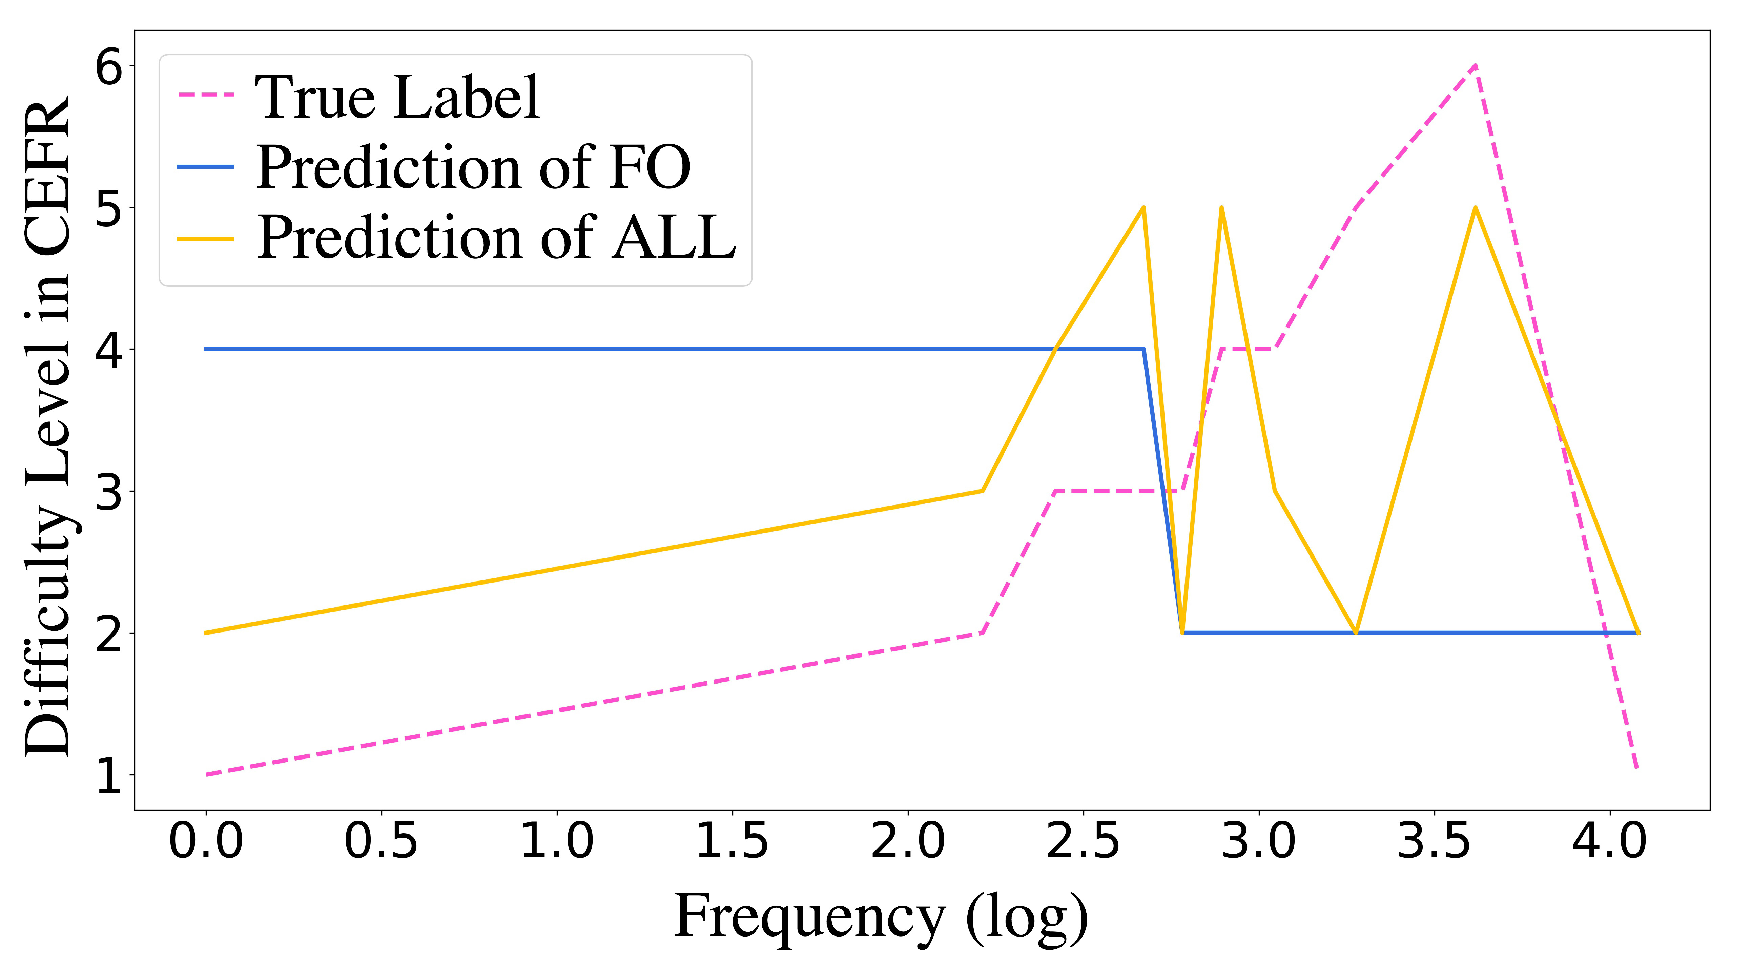
\includegraphics[width=1\linewidth]{pic/distance.eps} 
	\caption{The distribution of the ground truth and the prediction by FO and ALL.}
	\label{fig:distance}
\end{figure}
\begin{table}[th]
	\centering
	\scriptsize
	\begin{tabular}{|c|c|c|}
		\hline
		& \textbf{Pearson} & \textbf{Spearman} \\ \hline
		\textbf{Ground Truth\&FO} & -0.057 & -0.092 \\ \hline
		\textbf{Ground Truth\&ALL} & 0.305 & 0.300 \\ \hline
	\end{tabular}
\caption{\label{tab:coefficients} Correlation coefficient table.}
\end{table}

In German, our multi-faceted features have a better performance than human.
This result indicates that figuring out the difficulty levels manually with a short-time training is a truly difficult task. 
In English, the classification results of multi-faceted are very close to human accuracy. 
That is to say, our work is once again proven to be meaningful and there is still room for improvement.

	
